\documentclass[submission,copyright,creativecommons]{eptcs}
\providecommand{\event}{PLACES 2020} % Name of the event you are submitting to
%\usepackage{breakurl}             % Not needed if you use pdflatex only.

\usepackage{wrapfig}
\usepackage{graphicx}
\usepackage{subcaption}
\usepackage{stmaryrd}
\usepackage[strings]{underscore}
\usepackage{color}
\definecolor{purple}{rgb}{0.65, 0.12, 0.82}
\definecolor{darkgray}{rgb}{.4,.4,.4}

\usepackage{listings}
\lstdefinelanguage{Scribble}{
  keywords={module, type, from, as, global,protocol, role, to, choice, at, or, do},
  keywordstyle=\color{blue}\bfseries,
  identifierstyle=\color{black},
  sensitive=false,
  comment=[l]{//},
  morecomment=[s]{/*}{*/},
  commentstyle=\color{darkgray}\ttfamily,
  stringstyle=\color{purple}\ttfamily,
  morestring=[b]',
  morestring=[b]"
}
\lstdefinelanguage{JavaScript}{
  keywords={typeof, new, true, false, catch, function, return, null, catch, switch, var, if, in, while, do, else, case, break, class, export, boolean, throw, implements, import, this, const, let, extends},
  keywordstyle=\color{blue}\bfseries,
%  ndkeywords={class, export, boolean, throw, implements, import, this},
%  ndkeywordstyle=\color{darkgray}\bfseries,
  identifierstyle=\color{black},
  sensitive=false,
  comment=[l]{//},
  morecomment=[s]{/*}{*/},
  commentstyle=\color{darkgray}\ttfamily,
  stringstyle=\color{purple}\ttfamily,
  morestring=[b]',
  morestring=[b]"
}
\lstset{
	basicstyle=\footnotesize\ttfamily,
	numbers=left,
	frame=single,
}
\usepackage{caption}

\newcommand{\sectionref}[1]{\textsection~\ref{#1}}

\title{Verifying Interactive WebSocket Applications in TypeScript}
\author{Anson Miu
\institute{Imperial College London}
\and
Francisco Ferreira
\institute{Imperial College London}
\and
Nobuko Yoshida
\institute{Imperial College London}
\and
Fangyi Zhou
\institute{Imperial College London}
}
\def\titlerunning{Verifying Interactive WebSocket Applications in TypeScript}
\def\authorrunning{A. Miu, F. Ferreira, N. Yoshida \& F. Zhou}
\begin{document}
\maketitle

\begin{abstract}
Advancements in mobile device compute power has made interactive web applications possible, allowing the web browser to render content dynamically and support low-latency communication with the server. This comes at a cost to the developer, who now needs to reason more about the communication correctness of their application as they support more complex communication patterns. 

Multiparty session types (MPST) provide a framework for verifying implementations to conform to a prescribed communication protocol. Existing proposals for applying the MPST framework in application development either neglect the event-driven nature of web applications, or lack compatibility with industry tools and practices which discourage mainstream adoption by web developers.

In this paper, we present an implementation of the MPST framework for developing interactive web applications using familiar industry tools in TypeScript and the \textit{React.js} framework. The global communication protocol is specified in the Scribble protocol language and checked for well-formedness by the Scribble toolchain. We obtain the local protocol for each role, which describes the interactions of the global communication protocols observed by the role. We encode the local protocol into TypeScript types, catering for server-side and client-side targets separately, and show that our encoding guarantees that only implementations which conform to the protocol will type-check. We demonstrate the effectiveness of our approach through a web-based implementation of the classic \textit{Noughts and Crosses} game from a MPST formalism of the game logic.

\end{abstract}

\section{Introduction}
% Situation: stateful communication over WebSocket and interactive web applications

Modern interactive web applications aim to provide a highly responsive user experience by minimising the communication latency between clients and servers. 
Whilst the HTTP request-response model is sufficient for retrieving static assets, applying the same stateless communication approach for interactive use cases (such as a multiplayer game) introduces undesirable performance overhead from having to frequently set up new connections for client-server interactions. 
Developers have since adopted other communication transport abstractions over HTTP connections such as the WebSockets protocol \cite{WebSocketRFC} to enjoy low-latency full-duplex client-server communication in their applications over a single persistent connection. 
Enabling more complex communication patterns caters for more interactive use cases (such as real-time multiplayer games), but introduces additional concerns to the developer with respect to implementation correctness.

% Example: noughts and crosses
Consider a classic turn-based board game of \textit{Noughts and Crosses} between two players. Both players are identified by either noughts or crosses respectively, and take turns to place a mark on an unoccupied cell of a 3-by-3 grid until one player wins (when their markers form one straight line on the board) or a stalemate is reached (when all cells are occupied). A web-based implementation may involve players connected to a game server via WebSocket connections and interacting with the game from their web browser, which serve a \textit{single-page application} (SPA) of the game client written in a popular framework like \textit{React.js} \cite{React}. SPAs feature a single HTML page and dynamically renders content via JavaScript in the browser. Players take turns to make a move on the game board and the server implements the game logic to progress the game forward until a result (either a win/loss or draw) can be declared. 

Whilst WebSockets make this web-based implementation possible, it introduces the developer to a new family of communication errors, even for this simple game. In addition to the usual testing for game logic correctness, the developer needs to test against \textit{deadlocks} (e.g. both players waiting for each other to make a move at the same time) and \textit{communication mismatches} (e.g. player 1 sending a boolean to the game server instead of the board coordinates). The complexity of these errors, which correlate to the complexity of tests required against these errors, scale with the complexity of the communication patterns involved.

\textit{Multiparty Session Types} (MPST) \cite{MPST} provide a framework for formally specifying a structured communication pattern between concurrent processes and verifying implementations for correctness with respect to the communications aspect. By specifying the client-server interactions of our game as a protocol and verifying the implementations against the protocol for well-formedness, MPST theory guarantees well-formed implementations to be free from communication errors.

We see the application of the MPST methodology to verifying
interactive web applications written in TypeScript to be an
interesting design space -- to what extent can the MPST methodology be
applied such that we leverage TypeScript language features to maximise
static safety guarantees whilst preserving a flexible, natural and
idiomatic workflow for TypeScript developers? Such a workflow would
ultimately decrease the overhead for incorporating MPST into
mainstream web system, which reduces development time by
programmatically
verifying communication correctness of the implementation. 

\paragraph{Contributions}
This paper presents a workflow for developing type-safe interactive SPAs motivated by the MPST framework: \textbf{(1)} An endpoint API code generation workflow targeting TypeScript-based web applications for multiparty sessions; \textbf{(2)} An encoding of session types in server-side TypeScript that enforces static linearity; and \textbf{(3)} An encoding of session types in browser-side TypeScript using the React framework that guarantees affine usage of communication channels.

%Figure \ref{fig:workflow} illustrates our proposed development workflow: we extend the Scribble framework (\sectionref{section:scribble}) and generate TypeScript endpoints for server-side (\sectionref{section:server}) and browser-side (\sectionref{section:browser}) targets. We will use the \textit{Noughts and Crosses} game as our running example in the rest of the paper and show how our approach is a practical compromise that combines benefits from static session typing and being compatible with common libraries and idiomatic JavaScript practices (\sectionref{section:example}).

\section{The Scribble Framework}
\label{section:scribble}

Development begins by specifying the permitted communications between participants as a \textit{global protocol} in Scribble, a MPST-based framework introduced in \cite{Scribble} which features a protocol specification language and code generation toolchain. This means that a protocol specified in Scribble maps to some \textit{global type} in multiparty session type theory \cite{MPST}. We specify the \textit{Noughts and Crosses} game as a Scribble protocol in Listing \ref{lst:game}.

\begin{figure}[!h]
\begin{lstlisting}[
	language=Scribble
]
module NoughtsAndCrosses;
type <typescript> "Coordinate" from "./Types" as Point;	// Position on board

global protocol Game(role Svr, role P1, role P2) {
  Pos(Point) from P1 to Svr;
  choice at Svr {
    Lose(Point) from Svr to P2; Win(Point) from Svr to P1;
  } or {
    Draw(Point) from Svr to P2; Draw(Point) from Svr to P1;
  } or {
    Update(Point) from Svr to P2; Update(Point) from Svr to P1;
    do Game(Svr, P2, P1);
  }
}
\end{lstlisting}
\captionof{lstlisting}{Main body of the \textit{Noughts and Crosses} protocol.}
\label{lst:game}
\end{figure}

We leverage the Scribble toolchain to check for protocol
well-formedness. This directly corresponds to the multiparty session
type theory of verifying valid local type \textit{projections} for all
participants of a global type. The implementation of this validation
by the toolchain follows from the algorithmic projection procedures
defined in \cite{MPST}. We obtain a set of \textit{endpoint protocols}
-- one for each role from a well-formed global protocol. An endpoint protocol only preserves the interactions defined by the global protocol in which the target role is involved, and corresponds to an equivalent \textit{Endpoint Finite State Machine} (EFSM) in the Scribble toolchain. We use the EFSMs as a basis for API generation and adopt the formalisms in \cite{Hybrid2016}.


\section{Encoding Session Types in TypeScript}
% Design choices

Developers can validate the communication aspects of their
implementation against their EFSM to verify protocol conformance. Our
approach integrates the EFSM into the development workflow by encoding
session types as TypeScript types.
There are inherent differences between front- and back-end web development: business logic tends to initiate communication in the back-end, whilst communication in the front-end is mostly driven by user interactions with the browser. This motivates our design choice of generating different session types encodings for the target application on the server (\sectionref{section:server}) and in the browser (\sectionref{section:browser}).


\subsection{Server-side API generation}
\label{section:server}

\begin{wrapfigure}{r}{0.5\textwidth}
  \begin{center}
    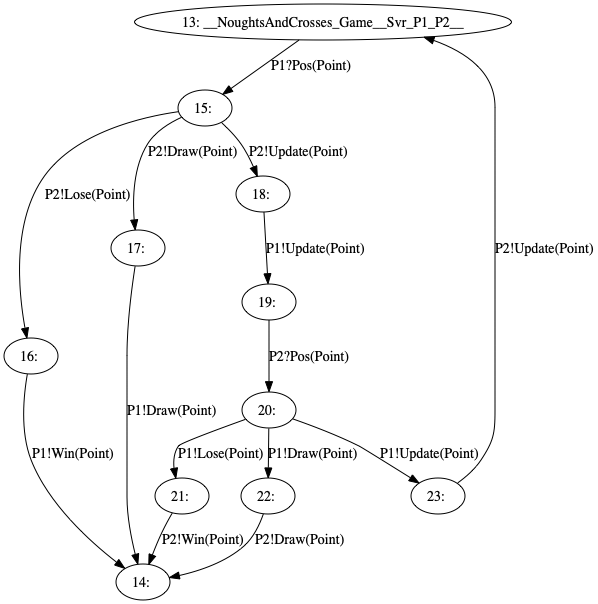
\includegraphics[width=0.48\textwidth]{figures/efsm_svr.png}
  \end{center}

  \captionof{figure}{EFSM for \texttt{Svr} in \textit{Noughts and Crosses}.}
  \label{fig:efsmsvr}
\end{wrapfigure}


We will refer to the \texttt{Svr} EFSM (fig.~\ref{fig:efsmsvr}) as a
running example in this section. For server-side targets, we encode
EFSM states as TypeScript types depending on the type of state. We
adopt the EFSM definition presented in \cite{Hybrid2016} to consider
receive and send states separately. Each TypeScript encoding is
assigned to its state identifier from the EFSM as its type alias, thus providing syntactic sugar when referring to the successor state in the TypeScript encoding of the current state. For any state $S$ in the EFSM, we refer to the TypeScript type alias of its encoding as $\llbracket S \rrbracket$. 

We make a key design decision \textit{not} to expose communication channels in the TypeScript session type encoding to provide linearity guarantees (\sectionref{section:serverlinear}). Our encoding sufficiently exposes seams for the developer to inject their business logic, whilst the generated session API (\sectionref{section:serversessionapi}) handles the sending and receiving of messages; as a result, the encoding does not concern with the role involved in the send/receive action. We outline the encoding below using examples from the \textit{Noughts and Crosses} game server (Listing \ref{lst:svr}).

\paragraph{Branching state} We consider a receive state as a unary branching state for conciseness. A branching state is encoded as an \textit{object literal} \cite{TypeScriptSpec}, with each branch corresponding to a member field. A branch expecting to receive a message labelled $\texttt{label}_i$ carrying payload of type $\texttt{T}_i$ with successor state $S_i$ is encoded as an \textit{member field} named $\texttt{label}_i$ of function type \texttt{(payload:$\texttt{T}_i$) => $\llbracket S_i \rrbracket$}. The developer implements a branching operation by passing callbacks for each branch, parameterised by the expected message payload type for that branch.

\paragraph{Selection state} We consider a send state as a unary selection state for conciseness. A selection state is encoded as a \textit{union type} \cite{TypeScriptSpec} of internal choice encodings: each internal choice sending a message labelled $\texttt{label}_i$ carrying payload of type $\texttt{T}_i$ with successor state $S_i$ is encoded as a \textit{tuple type} of \texttt{[Labels.label$_i$, T$_i$, $\llbracket S_i \rrbracket$]}. The developer implements a selection operation by passing the selected label and payload to send in the message. We generate a \textit{string enum} (named \texttt{Labels}) wrapping the labels in the protocol, hence the enum member access in the first element of the tuple type.

\begin{figure}[!h]
\begin{lstlisting}[language=JavaScript]
export type S13 = { Pos: (payload: Point) => S15 }
export type S15 = [Labels.Lose, Point, S16]
		| [Labels.Draw, Point, S17]
		| [Labels.Update, Point, S18]
\end{lstlisting}  
\captionof{lstlisting}{Example encodings from \textit{Noughts and Crosses} \texttt{Svr} EFSM.}
\label{lst:svr}
\end{figure}

\subsubsection{Session runtime}
\label{section:serversessionapi}

Our session runtime performs communication in a way that conforms to the protocol specification, but does not expose these IO actions to the developer by delegating the aforementioned responsibilities to an inner class. The runtime listens to message (receive) events on the communication channel, invokes the corresponding callback to obtain the value to send next, and performs the send. The developer instantiates the session by constructing an instance of the session runtime class.

\subsubsection{Linear channel usage}
\label{section:serverlinear}
Our callback-oriented design for server-side API generation provides guarantees on state channel linearity by preventing the two properties detailed below. Here, channel linearity is guaranteed based on the correctness of our library design and session runtime implementation, which means a faulty implementation could violate this, but is up to the library author to verify once rather than the end user.

\paragraph{Repeat use} We do not expose channels to the programmer, which makes \textit{reuse} impossible. For example, to send a message, the generated API only requires the payload that needs to be sent, and the session runtime performs the send internally, guaranteeing this action is done \textit{exactly once} by construction.

\paragraph{Unused} The initial state must be supplied to the session runtime constructor in order to instantiate the session; this initial state is defined in terms of the successor states, which in turn has references to its successors and so forth. This encoding approach will cover the terminal state (if it exists in the EFSM, as \cite{Hybrid2016} notes that an EFSM contains at most one terminal state), and the session runtime guarantees this terminal state, if it exists, will be reached by construction. 

\subsection{Browser-side API generation}
\label{section:browser}

We will refer to the \texttt{P1} EFSM (figure \ref{fig:efsmp1}) as a
running example in this section. Preserving behavioural typing and
channel linearity are known to be challenging for browser-side
applications due to the event-driven nature of user interaction: in
the case of \textit{Noughts and Crosses}, once the user makes a move
by clicking on a cell on the game board, this click event must be
deactivated until the user's next turn, otherwise the user can click
again and violate channel linearity. Our design goal is to enforce
this statically through the generated APIs. 

For browser-side targets, we extend the approach presented in \cite{MVU2019} on \textit{multiple model types} motivated by the \textit{Model-View-Update} (MVU) architecture. Each state in the EFSM is a model type and uniquely defines a \textit{view function}, set of \textit{messages} and \textit{update function}: the view function defines what to render to the DOM, the set of messages define the possible (IO) actions available at that state, and the update function defines which successor state to transition to, given some supported IO action at this state.


\begin{wrapfigure}{r}{0.5\textwidth}
  \begin{center}
    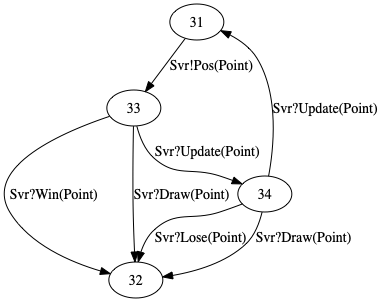
\includegraphics[width=0.48\textwidth]{figures/efsm_p1.png}
  \end{center}

  \captionof{figure}{EFSM for \texttt{P1} in \textit{Noughts and Crosses}.}
  \label{fig:efsmp1}
\end{wrapfigure}

\subsubsection{The React Framework}
Rather than using the LINKS web programming language from \cite{MVU2019}, we apply the multiple model types approach to the React framework \cite{React} developed by Facebook. React is widely used in industry to create scalable single-page TypeScript applications, and we intend for our proposed workflow to be beneficial in an industrial context. We introduce the key features of the framework below.

\paragraph{Components} A component is a reusable UI element which
contains its own markup and logic. Components implement a
\texttt{render()} function which returns a React element, the smallest
building blocks of a React application. Components can keep
\textit{state} and the \texttt{render()} function is invoked upon a
change of state. A simple counter can be implemented as a component,
with the count stored as state, a button which increments the count
when clicked and a \texttt{div} that renders the current
count. Components can also render other components, which gives rise
to a parent/child relationship between components. Parents can pass
data to children as \textit{props}: going back to the aforementioned
example, the the counter component could render a child component
\texttt{<StyledDiv count=\{this.state.count\} />} in its
\texttt{render()} function, propagating the \texttt{count} from its
state to the child. This enables reusability, and for our use case,
gives a control to the parent on what data to pass to its children (e.g. pass the payload of a received message to a child to render).

\paragraph{Virtual DOM (VDOM)} React components are rendered on a logical abstraction of the DOM, which in turn performs a \texttt{diff} on the current browser DOM and patches the delta accordingly. This allows the programmer to directly specify what should be rendered without having to worry about which elements to append or remove from the browser DOM.

\subsubsection{Model types in React}
We leverage React to express the model types approach in \cite{MVU2019} rather than the \textit{Model-View-Controller} (MVC) architecture it was intended for. 

\paragraph{State} An EFSM state is encoded as an \textit{abstract} React component. This is an abstract class to require the programmer to provide their own view function, which translates conveniently to the \texttt{render()} function of React components. Our session runtime (\sectionref{section:clientruntime}) ``executes'' the EFSM and renders the current state, so upon transitioning to a successor state, the successor's view function will be invoked, as per the semantics expressed in \cite{MVU2019}.

\paragraph{Model transitions} Transitions are encoded as React component props onto the encoded states by the session runtime (\sectionref{section:clientruntime}). We motivate the design choice of not exposing channel resources to provide guarantees on channel usage. React components in TypeScript are \textit{generics} \cite{TypeScriptSpec} which are parameterised by the permitted types of prop and state, which allows us to leverage the TypeScript compiler to verify that the props for model transitions stay local to the state they are defined for. The model transitions for EFSMs are message send and receive.

\subparagraph{Send} We make the assumption that message sending is triggered by some user-driven UI event (e.g. clicking a button, pressing a key on the keyboard) which interacts with some DOM element. We could pass a \texttt{send()} function as a prop to the sending state, but the programmer would be free to call the function multiple times which makes channel reuse possible. Instead, we pass a \textit{factory function} as a prop, which will, given an HTML event and a event handler function, return a fresh React component that binds the sending action on construction, so once the bound event is triggered, our session runtime executes the event handler function to obtain the payload to send, perform the send \textit{exactly once} and transition to (which, in practice, means render) the successor state. 

\begin{figure}[!h]
\begin{lstlisting}[language=JavaScript, tabsize=4]
// Inside some render() function..
{board.map((row, x) => (
	row.map((col, y) => {
		const SelectPoint = this.props.Pos('click', (event: UIEvent) => {
			event.preventDefault()
			return { x: x, y: y }}
		return <SelectPoint><td>.</td></SelectPoint>
})}
\end{lstlisting}  
\captionof{lstlisting}{Model transition for message sending in 
\textit{Noughts and Crosses} \texttt{P1} implementation.}
\label{lst:clientapp}
\end{figure}

We clarify the semantics using the \textit{Noughts and Crosses} example in Listing \ref{lst:clientapp}. \texttt{this.props.Pos} is the factory function prop passed from the session runtime. For each x-y coordinate on the game board, we create a \texttt{SelectPoint} React component from the factory function (which reads ``build a React component that sends the \texttt{Pos} message with x-y coordinates as payload when the user clicks on it'') and we wrap a table cell (the game board is rendered as a HTML table) inside the \texttt{SelectPoint} component to bind the click event on the table cell.

\subparagraph{Receive} The payload of a message receive transition is passed as a prop to the successor state and can be handled in the successor's view function. Upon receiving the message from the channel, the session runtime renders the successor of the receive state and propagates the payload as the prop accordingly.

\subsubsection{Session runtime}
\label{section:clientruntime}

Our session runtime can be interpreted as an abstraction on top of the React VDOM that implements the EFSM by construction. The session runtime itself is a React component too, named after the endpoint role identifier: it opens the WebSocket connection to the server, keeps track of the current EFSM state as part of its React component state, and most importantly, renders the React component encoding of the active EFSM state. Channel communications are managed by the runtime, which allows it to render the successor of a receive state upon receiving a message from the channel. Similarly, the session runtime is responsible for passing the required props for model transitions to EFSM state React components. The session runtime component is rendered by the programmer and requires the following props:

\paragraph{Endpoint URL} The session runtime needs this in order to open the WebSocket connection.

\paragraph{Concrete state components} The programmer writes their own implementation of each state (mainly to customise how the state is rendered and inject business logic into state transitions) by extending the abstract React class components. The session runtime requires references to these concrete components order to render the user implementation accordingly.

\subsubsection{Affine channel usage}
A limitation of our browser-side session type encoding is only being able to guarantee that channel resources are used \textit{at most once} as supposed to \textit{exactly once}.

Communication channels are not exposed to the programmer so multiple sends are impossible. This does not restrict the programmer from binding the send action to exactly one UI event: for the \textit{Noughts and Crosses} game, we bind the \texttt{Pos(Point)} send action to each unoccupied cell on the game board, but the generated runtime ensures that, once an event bound to the send action is triggered, the send is only performed once and the successor state is rendered on the DOM to prevent multiple sends initiated by the user.

However, our approach \textit{does not} statically detect whether all transitions in a certain state are bound to some UI event. This means that it is possible for an implementation to \textit{not} handle transitions to a terminal state but still type-check, so we cannot prevent unused states.

\section{Case Study}
\label{section:example}

\begin{figure}
\begin{lstlisting}[language=JavaScript, tabsize=4]
const handleP1Move: Receive_P1 = (move: Point) => {
	// User-implemented logic
	board.P1(move)
	if (board.won()) { return [Labels.Lose, move, move] }
	else if (board.draw()) { return [Labels.Draw, move, move] }
	else { return [Labels.Draw, move, handleP2Move] } 
}

const handleP2Move: Receive_P2 = ...

// Instantiate session
new NoughtsAndCrosses.Svr(webSocketServer, handleP1Move, handleP2Move)
\end{lstlisting}  
\captionof{lstlisting}{Example fragment of \textit{Noughts and Crosses} \texttt{Svr} implementation.}
\label{lst:svrprotocol}
\end{figure}

We apply our framework to implement a web-based implementation of the \textit{Noughts and Crosses} running example in TypeScript; the interested reader can find the full implementation in \cite{NoughtsAndCrosses}. In addition to MPST-safety, we show that our library design welcomes idiomatic JavaScript practices in the user implementation and is interoperable with common front- and back-end frameworks.
 
\paragraph{Game server} We set up the WebSocket server inside an Express.js \cite{ExpressJS} application on top of a Node.js \cite{NodeJS} runtime. We define our own game logic in a \texttt{Board} class to keep track of the game state and expose methods to query the result. This custom logic is integrated into our \texttt{Receive\_P1} and \texttt{Receive\_P2} handlers (Listing \ref{lst:svrprotocol}), so the session runtime can handle \texttt{Pos(Point)} messages from players and transition according to the injected game logic. 

Note that, by the structural typing nature of TypeScript, replacing \texttt{handleP2Move} on line 6 with \texttt{handleP1Move} would be type-correct - this allows for better code reuse as supposed to defining additionl abstractions to work around the limitations of nominal typing in \cite{Hybrid2016}. There is also full type erasure when transpiling to JavaScript to run the server code, so state space explosions is never a runtime consideration.

\paragraph{Game clients} We implement the game client for players as a React application - extending from the generated abstract React components, registering our custom implementation as props for the session runtime component.

For the sake of code reuse for demonstration purposes, \cite{NoughtsAndCrosses} uses \textit{higher-order components} (HOC) to build the correct state implementations depending on which player the user chooses to be. We leverage the \textit{Redux} state management library to keep track of game state, thus showing the flexibility of our library design in being interoperable with other libraries and idiomatic JavaScript practices. 

\section{Related Works}
%\paragraph{Languages with native session type support} \dots
% New languages written  (e.g. ATS)
%	- addresses the challenge of resource linearity with a liner type system
%	- problem with webdev: not compatible with libraries, technologies, flexibility of JavaScript (ultimately the language of the browser)

\paragraph{Endpoint API generation} \cite{Python2017} targeted Python applications and the generation of runtime monitors to dynamically verify communication patterns. Whilst the same approach could be applied to JavaScript, we can provide more static guarantees with TypeScript's gradual typing system and compiler. \cite{Hybrid2016} targeted Java applications and proposed to encode the EFSM states and transitions as classes and instance methods respectively, with behavioural typing achieved statically by the type system and channel linearity guarantees achieved dynamically since channel resources are exposed and aliasing is not monitored.

\paragraph{Session types in web development} \cite{PureScript2019} targeted web development in PureScript using the \textit{Concur UI} framework and proposed a type-level encoding of EFSMs as multi-parameter type classes. However, it presents a trade-off between achieving static linearity guarantees from the type-level EFSM encoding under the expressive type system and providing an intuitive development experience to programmers, especially given the prevalence of JavaScript and TypeScript applications in industry. \cite{MVU2019} focused on applying binary session types in front-end web development and presented approaches that tackle the challenge of guaranteeing linearity in the event-driven environment. 

Our work applies the aforementioned approaches in a \textit{multiparty} context in a manner that is compatible with industrial tools and practices to ultimately invite the notion of MPST-safety into interactive web application development in industry.

\section{Conclusion and Future Works}
We have presented a MPST-based framework for developing full-stack interactive TypeScript applications with WebSocket communications that conform to a protocol, statically providing linear channel usage guarantees and affine channel usage guarantees for back-end and front-end targets respectively.

Future works include incorporating \textit{explicit connection actions} introduced in \cite{ExplicitConnections} in our API generation to better model real-world communication protocols that may feature in interactive web applications. Whilst our approach does support multiparty sessions, protocols are required to have exactly one role running on the server and client roles must interact with each other via the server to respect the properties of WebSocket connections, which is the transport abstraction we support. Extending support to WebRTC would cater for peer-to-peer communication between browsers, which further opens up possibilities for communication protocols supported by our approach.

% Future work
% - generalise to encode protocols as typestates (e.g. Mungo example)
% - WebRTC for full MPST (since current limitation is w.r.t. MPST protocols with 1-server many-client roles

\nocite{*}
\bibliographystyle{eptcs}
\bibliography{generic}
\end{document}
